%************************************************
\chapter{Introduction}\label{ch:intro}
%************************************************


\section{Life history and responses to environmental changes}

At the most fundamental level, the persistence of population hinges on the fate
of individuals surviving and reproducing in their environments \citep{Sol2016}.
If individuals
are able to reproduce at a higher rate than they die, the population will
increase in numbers and persist over time; if the balance is negative, however,
the population will decrease over time and end up extinct.
Because the rates of birth and death are ultimately determined by how
organisms allocate their limited time and energy to reproduction and survival
\citep{stearns1992evolution}, life history theory has long been deemed essential
to understanding the dynamics of populations \citep{Saether2004, Sol2012a}.

Concern over the loss of biodiversity associated with human-induced rapid 
environmental alterations has generated an urgent need to understand why
organisms differ in their response to environmental changes.


\begin{small}
\begin{framed}
\subsection*{Box 1: Life History}
Life history strategies are the different ways in which organisms allocate the
limited resources among different components of fitness such as reproduction,
survival and development \citep{stearns1992evolution,roff2002}⁠.
Thus, each strategy is defined by a combination of life history traits such as
clutch size, broods per year, age at first breeding or lifespan
\citep{Violle2007}⁠.
Mechanisms that generate the trade-offs explaining the observed covariance
among traits include resource partitioning, correlational selection between
traits and antagonistic pleiotropy \citep{Roff2007, Stearns1989a}.
Incompatible physiological states mediated by the endocrine system
\citep{Ricklefs2002}⁠ generate another source of mechanisms linking life
history traits mediated by behaviour \citep{Reale2010a}.

There is a consensus on the general features of a plausible explanation for the
evolution of life history traits \citep{Stearns2000}⁠: (1) life histories
are shaped by the interaction of extrinsic and intrinsic factors, (2) the
extrinsic factors are ecological impacts on survival and reproduction; (3) the
intrinsic factors are trade-offs among life history traits and lineage-specific
constraints on the expression of genetic variation.
\end{framed}
\end{small}


Despite the solid foundations and appealing logic behind the life history
theory, no conclusive patterns linking the live history and the responses to
environmental changes have been described. This is one of these strongholds
that science has laid siege to, but has never completely conquered and perhaps a
more holistic approach can help to overcome \citep[p.~269--274]{levins1985}.
Life history theory covers a huge range of levels of organisation, from genetics
at individual level to demography, including the effects of the environment and
other species in the ecosystem. Furthermore, life history affects and is
affected by the processes at each level of organisation (see figure
\ref{fig:fig1.1}). Most of the works framed in the life history theory focus on
few levels (reviewed in \citet{Stearns2000}).


\begin{figure}
\centering
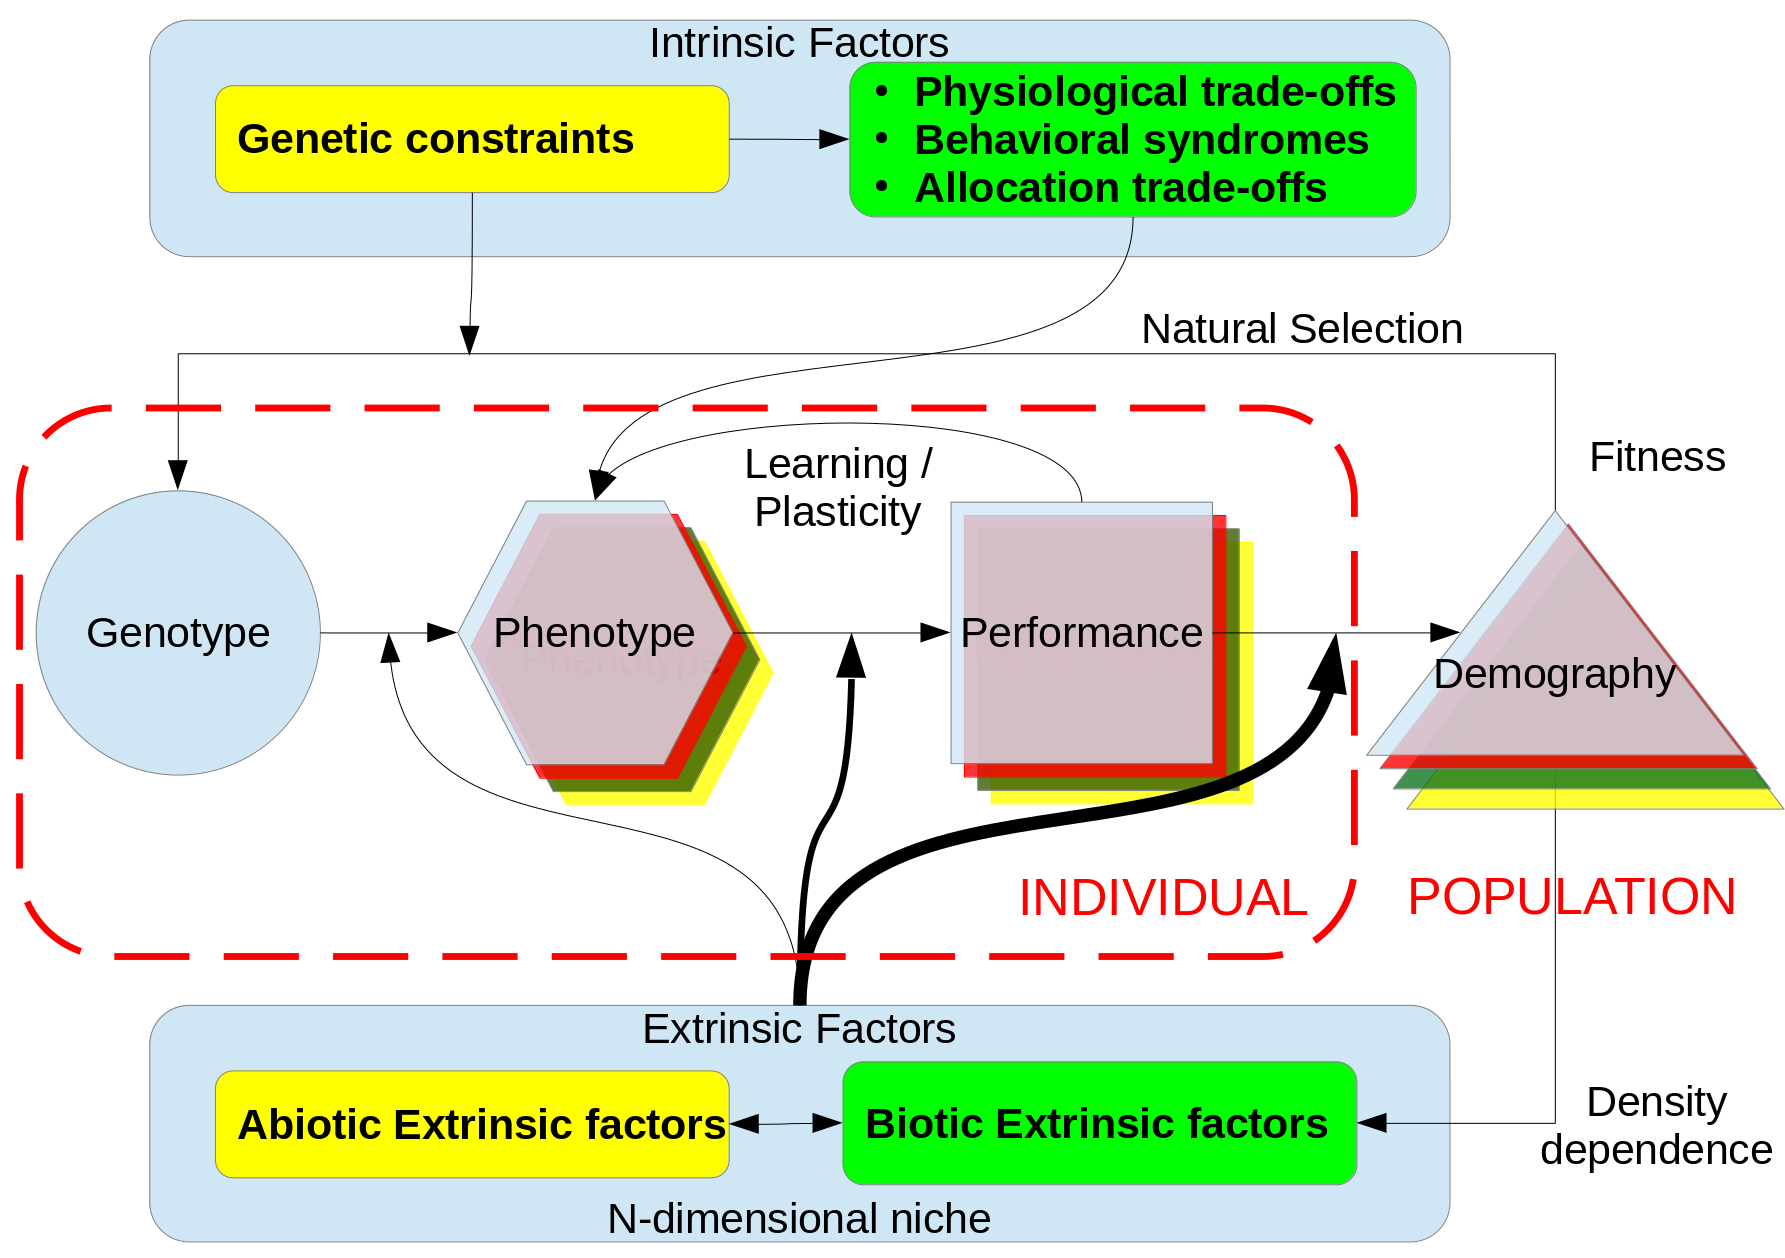
\includegraphics[width=\textwidth]{./Figures/intro/esquemaLH.png}
\caption[LH schema]{
Schematic representation of the life history theory framework with the
different levels of organisation and their relations.
The life history of an individual depends on a series of steps from the
genotype to the phenotype, which then interacts with the environment resulting
in a specific performance in terms of reproduction and survival. The effect of
the environment exerts a greater influence at each step modifying the phenotype
and the performance of the individuals and ultimately, at the population level,
modifying the fitness and the age structure.
At the same time, differential fitness among genotypes changes their frequency
in the population by natural selection resulting in evolutionary change. A
second feedback in the system is the influence of organisms and population
on the environment by modifying the population density for the same
species or other species being relevant such as preys or predators. Any change
modifying the age-specific mortality will result in a change in the optimum
life history strategy. Inspired by \citet{Ricklefs2002}.
}
\label{fig:fig1.1}
\end{figure}


Despite the seductive philosophy described by \citet{levins1985}, pragmatism and
the need to put limits to this thesis impose to focus on a subset of the
framework. I choose to focus on phenotype and demography.
To characterise the phenotype I use life history traits, individual traits
with direct effects on fitness such as clutch size, age at first breeding or
number of broods per year. I do not consider intraspecific variation, but the
traits were aggregated at species level throughout this thesis.
The demographic traits are the population level features affecting
the growth rate such as age-specific mortality rate or average fecundity and
also were aggregated at species level. Neither evolution nor temporal variation
were considered for the life history traits or for demographic traits.
Regarding the environmental change, I used data to compare urban and non-urban
areas (Chapter \ref{ch:POLS}) and simulated the effects of unknown new
habitats or resources with better or worst juvenile or adult survival (Chapter
\ref{ch:LH-Behaviour model}).


\section{Life history and behavior}

Behaviour mediates how animals interact with their environment and, by virtue
of their plastic nature, it can modify the nature of these interactions, shaping
the biotic and abiotic pressures that act upon them
\citep{Futuyma1988,Losos2004,Lapiedra2013}. The idea that behaviour, through
cognitive and neural machinery, allows behavioural solutions to unusual or new
problems to be devised is known as the cognitive buffer hypothesis
\citep{Allman1993,VanSchaik2003,Sol2009,Sol2009a}.


\begin{small}
\begin{framed}
\subsection*{Box 2: Behavioral Plasticity}

Behaviour can be defined as the actions or inactions of organisms that change
their relation with the environment as a response to external or internal
stimuli. As such, it is a form of phenotypic plasticity. We can distinguish two
types of behavioral plasticity: activational and developmental plasticity.

\subsubsection*{Activational Plasticity}

Activational plasticity refers to the expression of behaviour and describes the
innate response to stimuli that triggers a shift to an alternative behaviour
through the activation of a neural network \citep{Snell-Rood2013}. Because of
its immediacy and reversibility, such forms of plasticity allow individuals to
rapidly respond to environmental uncertainties by enabling rapid modulation
of, or transitions between, behaviours as a function of the individuals’ needs
\citep{Snell-Rood2013,Sol2013a}. This kind of pre-established responses can be
maladaptive if the individuals face new conditions for which no evolutive
selection has taken place, leading to a so called ecological traps
\citep{Kokko2001}.

\subsubsection*{Developmental Plasticity}

Animals can confront novel challenges, like the need to obtain new types of food
or avoid unfamiliar predators, by modifying or inventing new behaviours, a
process known as developmental behavioural plasticity \citep{Snell-Rood2013}.
Developmental behavioural plasticity is not so immediate as activational
plasticity, because it involves changes in the nervous system that alter motor
responses. However, it has the advantage that it allows animals to construct
responses to unfamiliar or novel problems. One of the main mechanisms behind
developmental behavioural plasticity is learning, the acquisition of new
information influencing performance in behaviour \citep{Dukas1998}. Instead of
consistently expressing the same behaviour to a particular stimulus, learning
allows animals to devise innovative behavioural responses or to improve already
established behaviours on the basis of experience
\citep{Lefebvre1997,Dukas1998,Reader2002,VanSchaik2003,Ricklefs2004}. Learning
is particularly relevant in facilitating the responses to environmental changes,
including new resources, predators or habitats.
\end{framed}
\end{small}


As I argue in this thesis, if we want to fully understand how life history
affects the population dynamics of animals exposed to environmental changes, we
need to explicitly consider the role of behaviour. The argument for the need
to better integrate behaviour into life history theory is founded upon three
main principles.
The first is the fact that behavioural responses are part of the adaptive
machinery of animals to cope with uncertainties and evolutionary disequilibria
of novel environments. While the idea is not new \citep{mayr1965}, recent
theoretical and empirical advances provide a strong foundation for moving
forward \citep{Sol2020, Ducatez2020}.
The second argument is the growing evidence that behaviour affects and is
affected by life history, which implies that both are part of a same adaptive
strategy \citep{Ricklefs2002,Reale2010a,Sol2016,Sol2016a}. When behaviour
changes the relations of the individuals with the environment, the age-specific
mortality and therefore the optimum life history strategy also change. Thus,
when we examine how life history affects population dynamics, including
extinction or colonization, we are considering not only life history mechanisms
but also mechanisms related to behavioural responses to novel environments
\citep{Sol2016}.
The third and last argument is that behaviour mediates some life history
mechanisms of response to novel environments, particularly those related to
environmental uncertainty and adaptive mismatch. For example, to breed or not
to breed is a behavioural decision with direct effects in the number of eggs
produced in a year.
By clearly delineating these mechanisms, we can better infer when it is
necessary to consider behaviour to understand how life history affects the
response to environmental changes.


\section{Objectives}

In my thesis I addressed fundamental unresolved questions about the 
interaction of life history and behaviour in facilitating or impeding the 
response to rapid environmental changes. Chapter \ref{ch:LHaxes} describes the 
main axes of life history traits variation in birds using a demographic
approach within a phylogenetic comparative framework. Chapters
\ref{ch:LH-Behaviour model} and \ref{ch:POLS} explore the links between life
history and behavior, the first using a theoretical model focused on the process
of colonization of novel environments to better understand the mechanisms, and
the second analysing empirical data using comparative methods from urban and
non-urban populations looking for patterns relating life histories and behavior.
The specific goals of the chapters are:


\begin{itemize}
\item \textbf{Chapter \ref{ch:LHaxes}: To describe the axes of life history 
variation in birds}

Not all combinations of life history traits exists in nature. Traits covary
due to trade-offs and are organized among different axes. A major axis
of variation of the life history traits is the so-called fast-slow continuum,
which mainly reflects a fecundity-survival trade-off. However, defining and
quantifying the fast-slow axis has proven to be difficult and at least 18
studies have attempted to characterise the fast-slow axis in the last 40 years
with no clear consensus regarding the life history traits that best define it.
I tried to address this problem by giving a demographically meaningful
definition to the axis and identifying the combination of traits that better
describe the underlying trade-off.
In this chapter, I defined the fast-slow axis that better predicts the 
elasticity of the adult survival and generation time from available demographic 
models and a large dataset of life history traits of birds, and describe other
less studied axes of life history from the remaining variation such as the
degree of iteroparity, the relative egg size or the lifelong productivity. Then,
I generated a a global dataset for birds with the position of each species along
the new fast-slow axis, which then can be used for comparative analyses (see
Chapter \ref{ch:POLS} for example).
\bigskip


\item \textbf{Chapter \ref{ch:LH-Behaviour model}: To explore the mechanisms 
linking life history and behavior}

I developed a theoretical individual based model simulating the introduction of
a species with different life histories in a new environment with different
habitat options characterized by different degrees of habitat mismatch that
affects adult or juvenile mortality and evaluate how the life history and
behaviour could interact and affect the persistence of the population under
stochastic and maladaptive scenarios. Specifically, I tested 6 different
behaviours representing activational plasticity affecting preferences for the
best habitat or the worst (ecological trap) or skipping a reproductive event
when individuals are on the worst habitat, and behaviours representing
developmental plasticity by increasing the probability to change habitat
when there is a breeding failure or by learning by exploring, and a neutral
choice behavior.
\bigskip


\item \textbf{Chapter \ref{ch:POLS}: To analyse the effects of life history and 
behaviour in the ability to colonize urban habitats}

By means of a comparative analysis of flight initiation distances (i.e., the
distance at which an animal takes flight when a human being is approaching)
across \textgreater{300} bird species distributed worldwide, I show the
existence of a peace-of-life syndrome (POLS) predicted by theory where
slow-lived species tend to be more risk-averse than fast-lived species.
Furthermore, the POLS structure vanishes in urbanized environments due to
slow-lived species adjusting their flight distances based on the perception of
risk. The results shows that slow species have a more plastic behaviour which
can potentially facilitate the adaptation to environmental changes.
\end{itemize}

\bigskip


I believe that this thesis will contribute to develop a new way to understand
how life history influences population growth in novel or changing environments,
potentially contributing to a more predictive theory. Such a theory may be
useful to help prevent and mitigate the ecological and economic impact of
biological invasions \citep{Kolar2002, Vall-llosera2009, Leung2012}. The new
theory should also be of great importance in predicting extinction risk
associated with human-induced rapid environmental changes like habitat
destruction and climate change \citep{Saether2000, Sih2011}.
